\begin{figure*}[ht]
  
  \begin{subfigure}{.315\textwidth}
    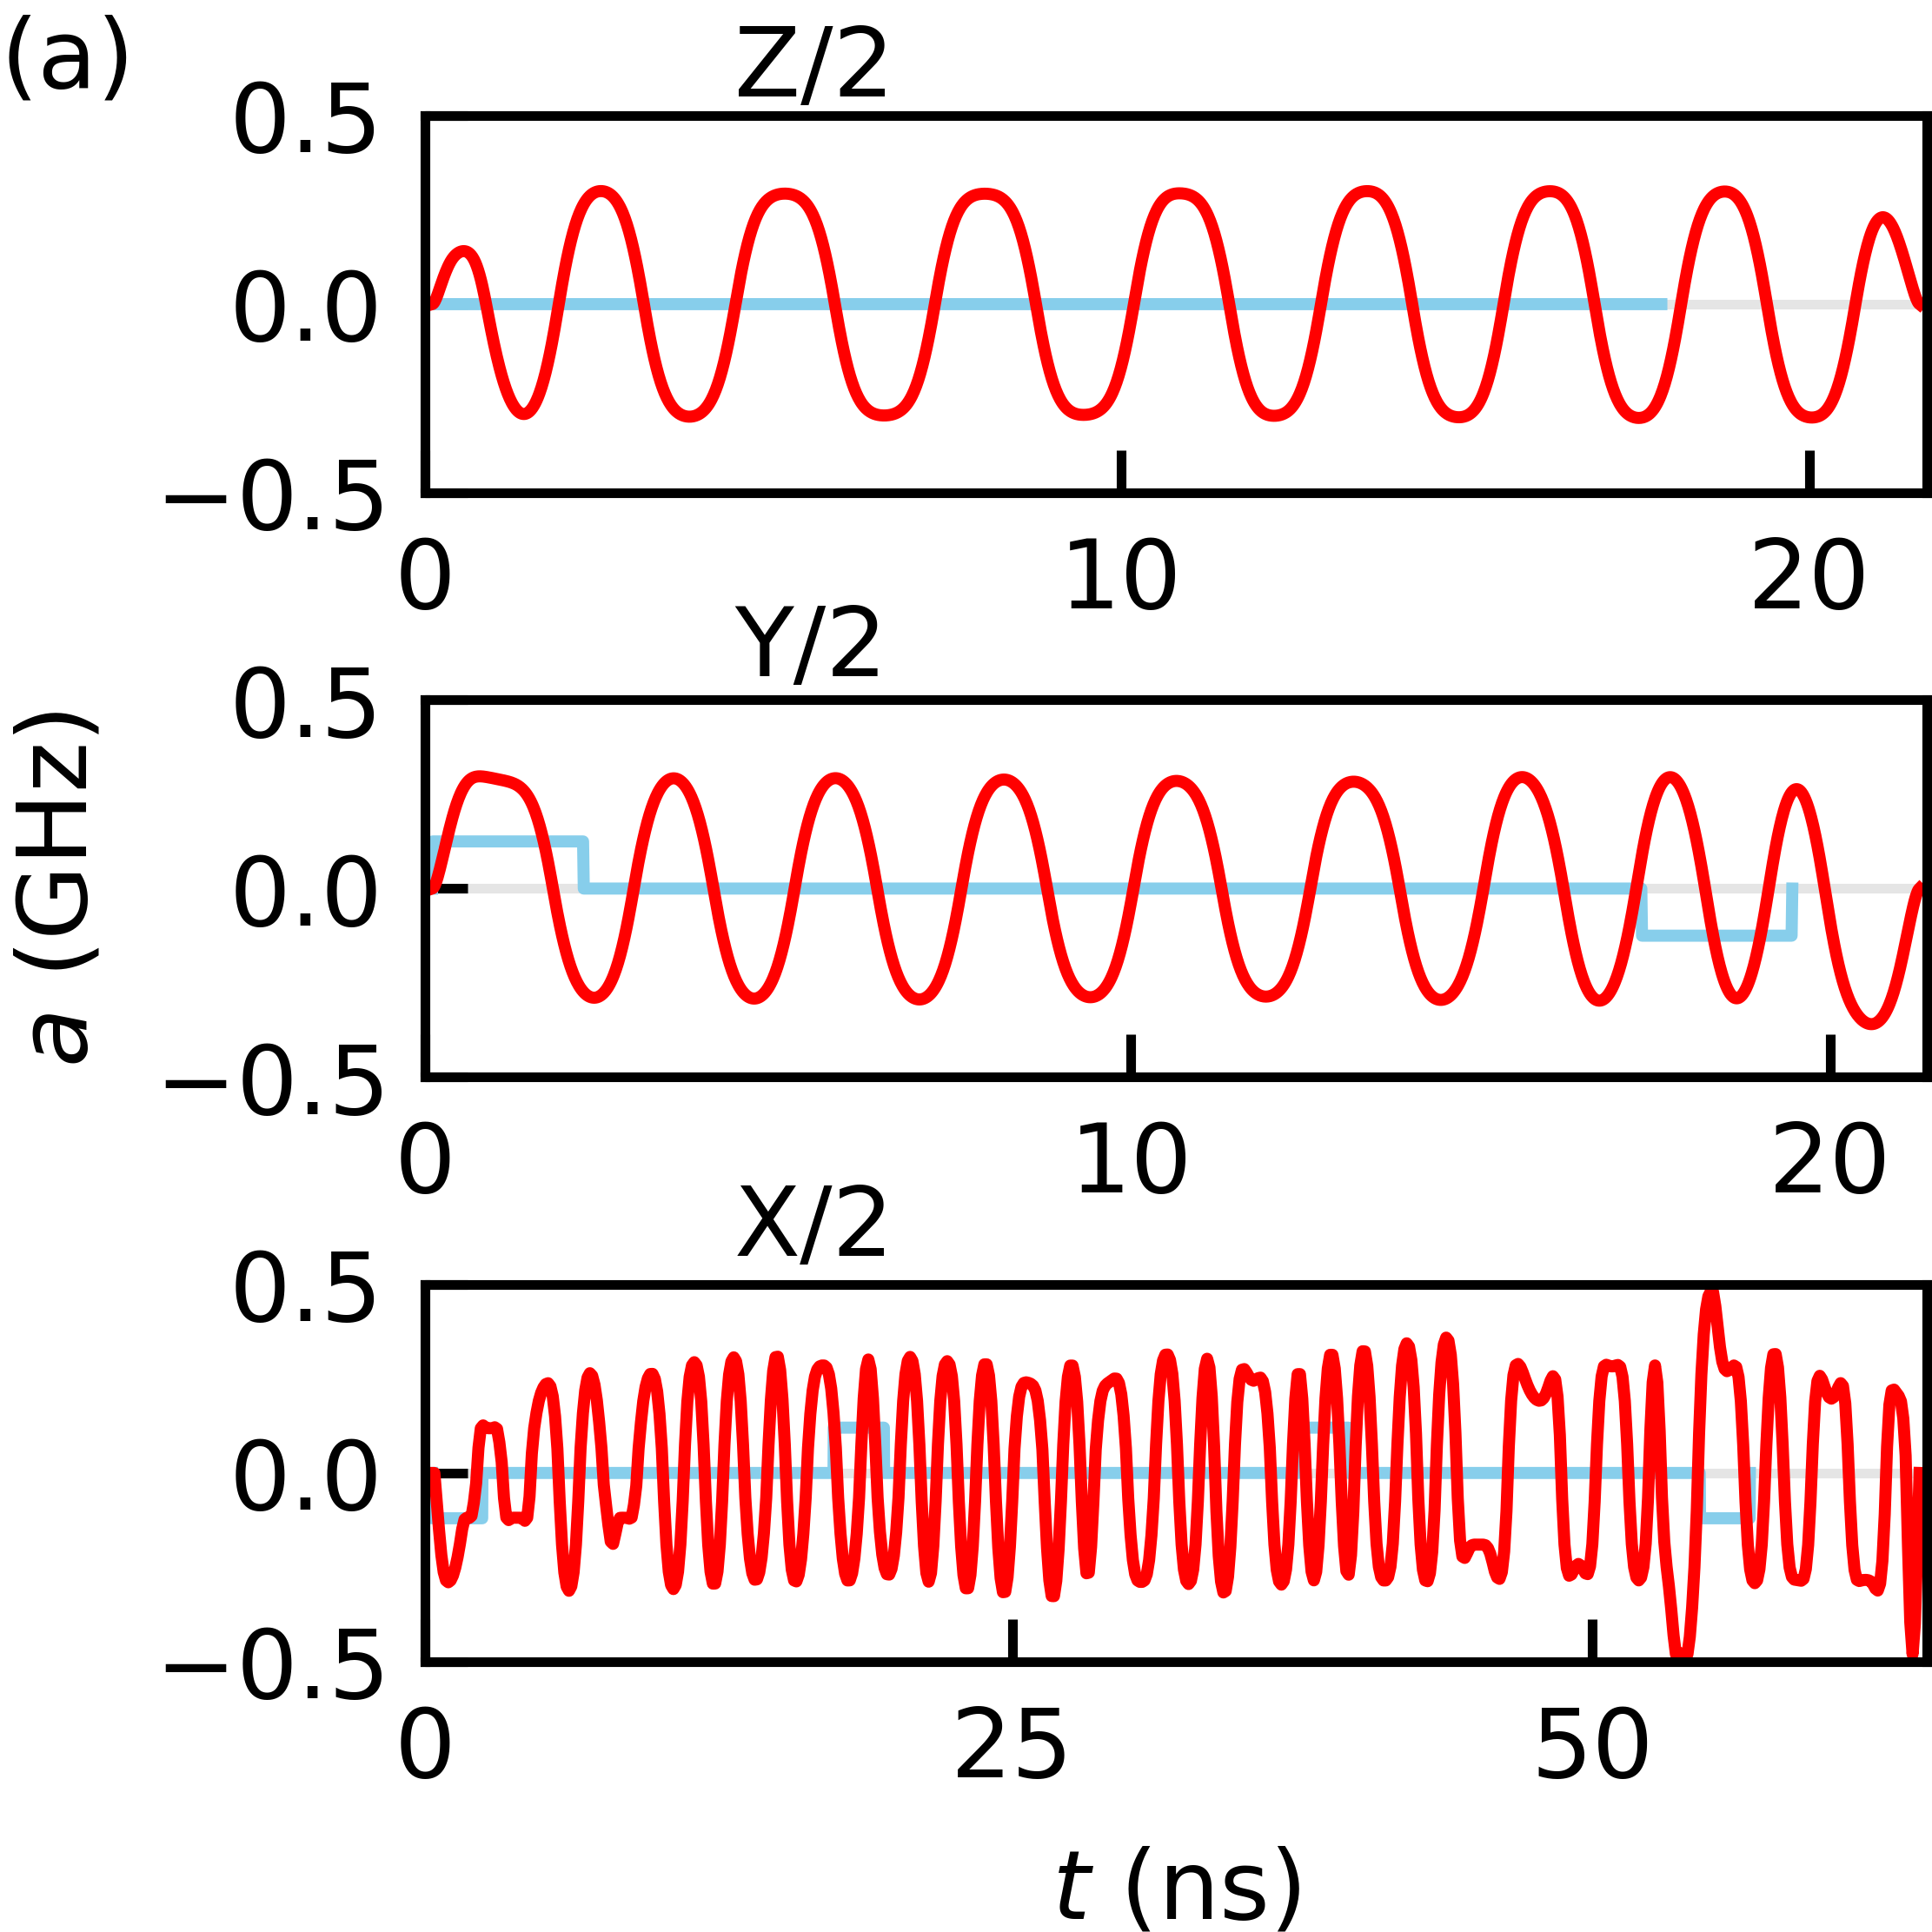
\includegraphics[width=\linewidth]{assets/f1a.png}
  \end{subfigure}\hfill
  \begin{subfigure}{.23\textwidth}
    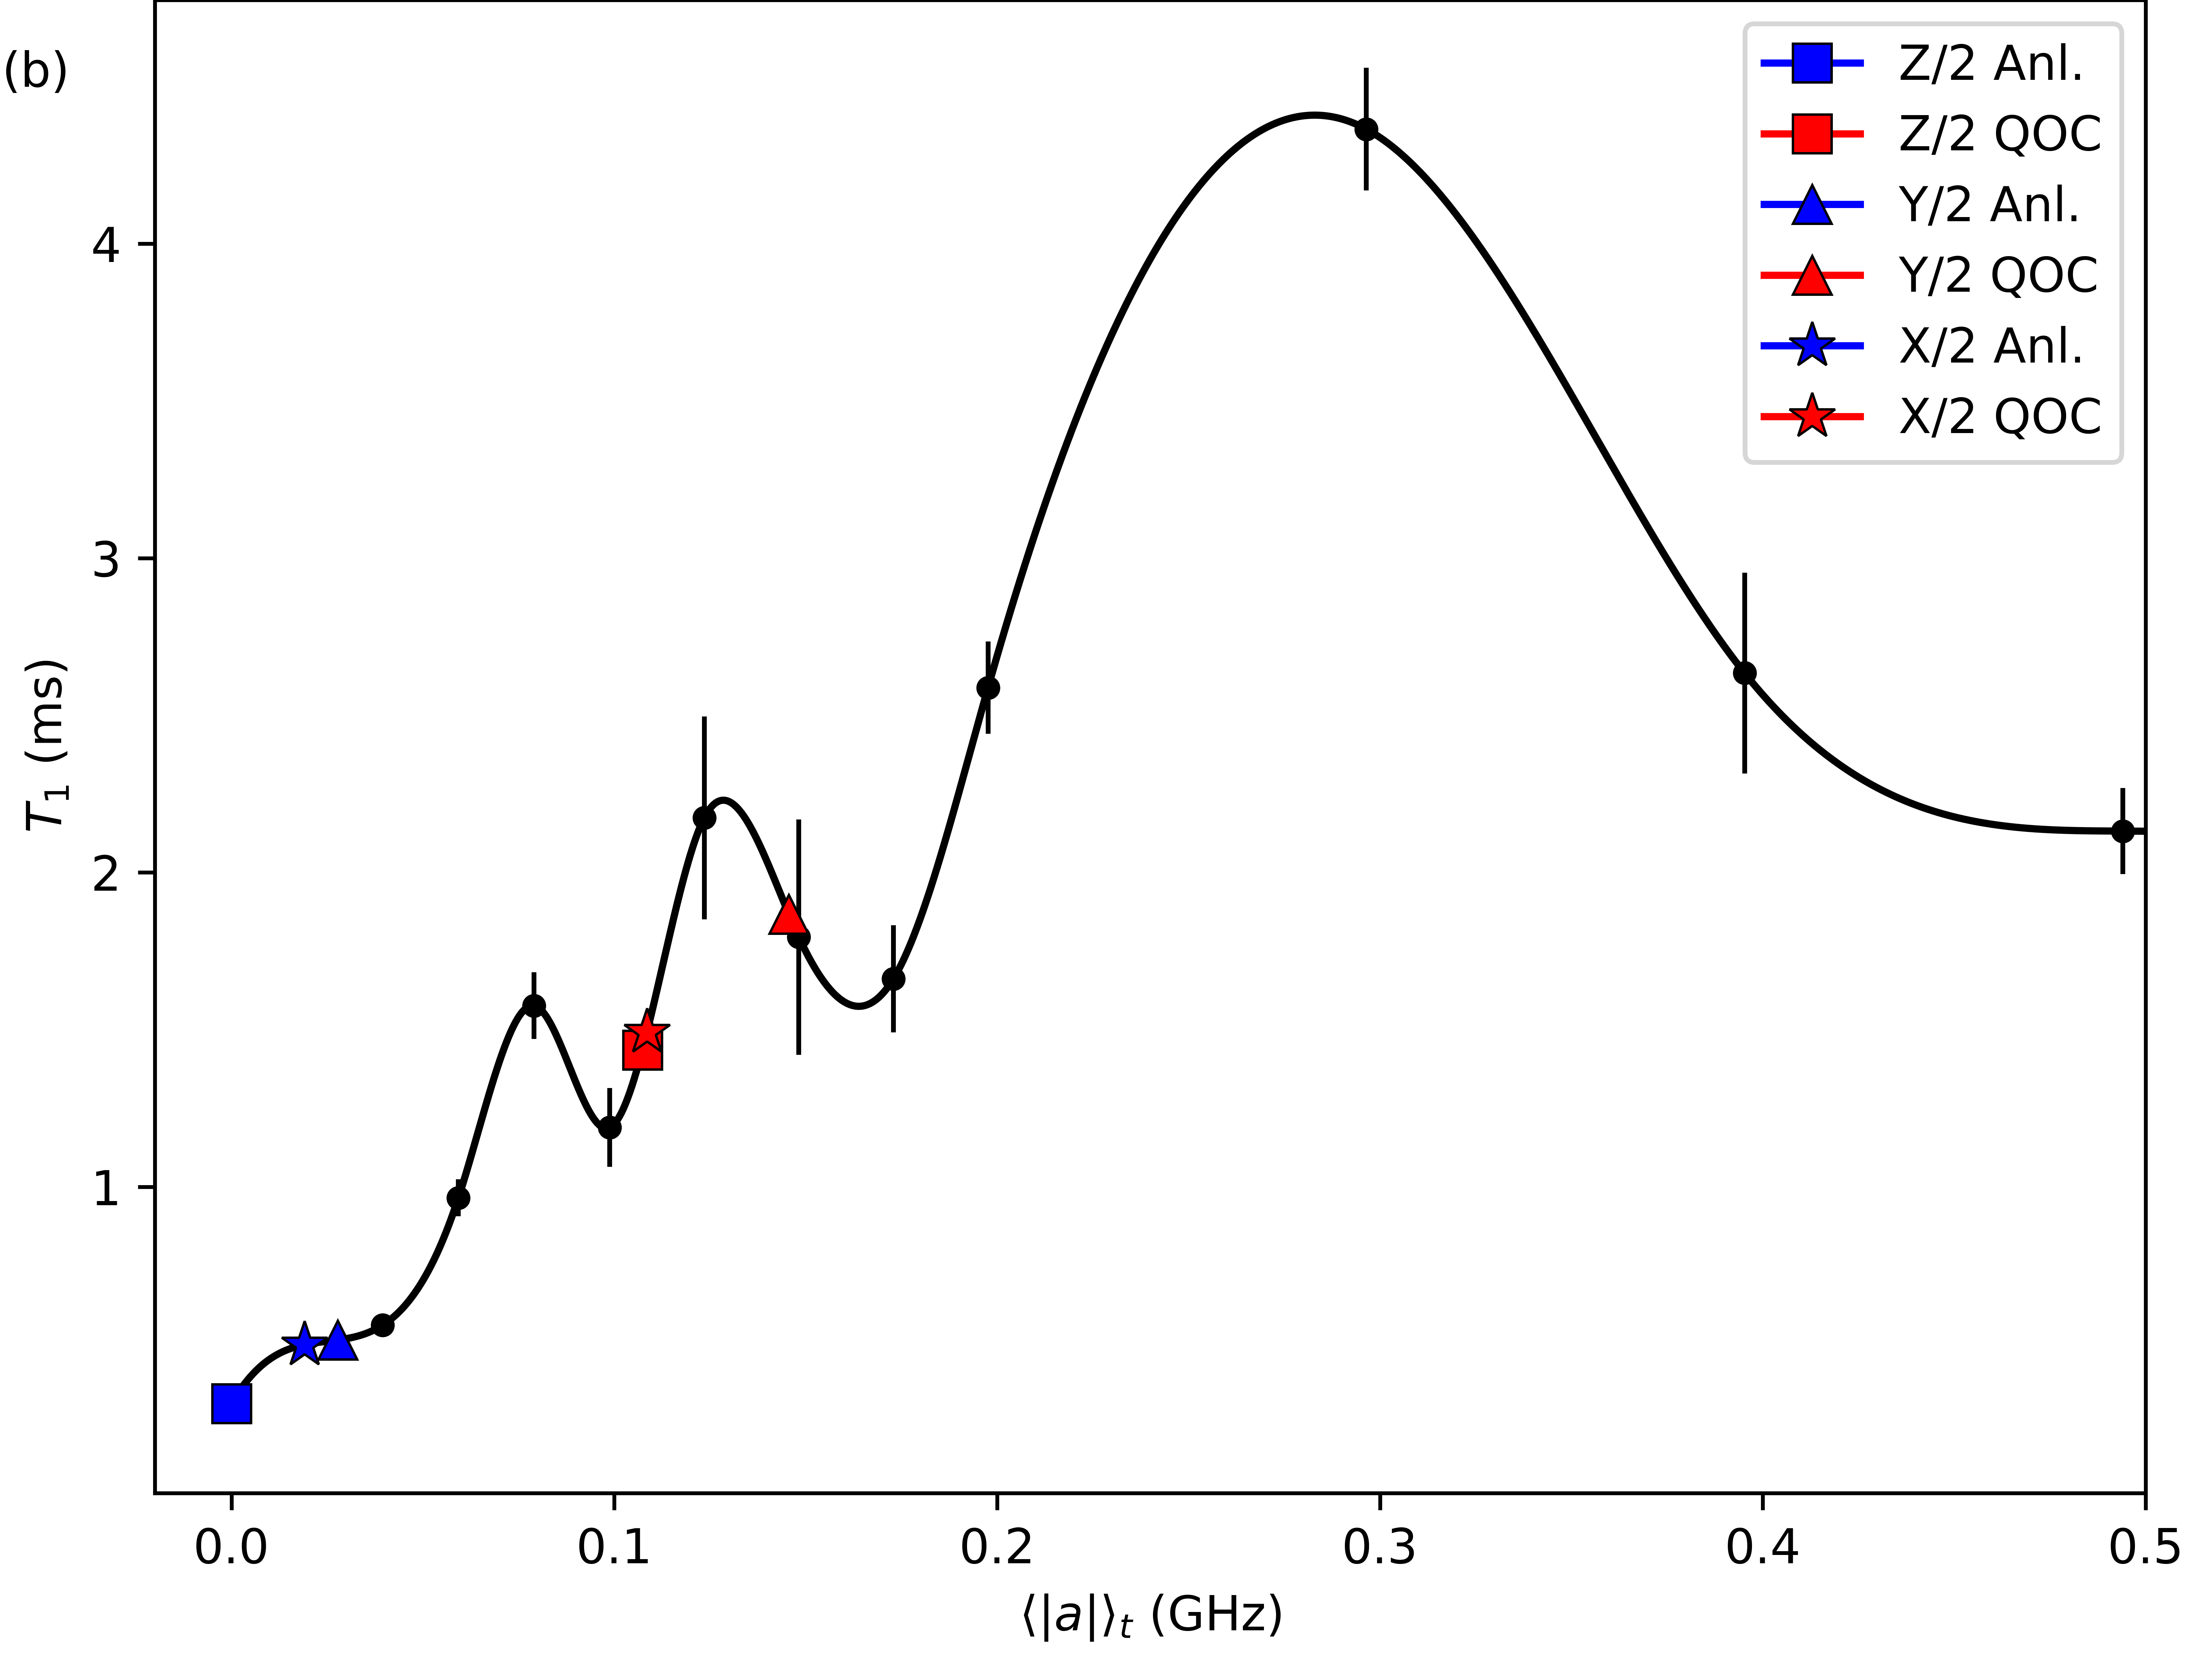
\includegraphics[width=\linewidth]{assets/f1b.png}
  \end{subfigure}\hfill
  \begin{subfigure}{.4\textwidth}
    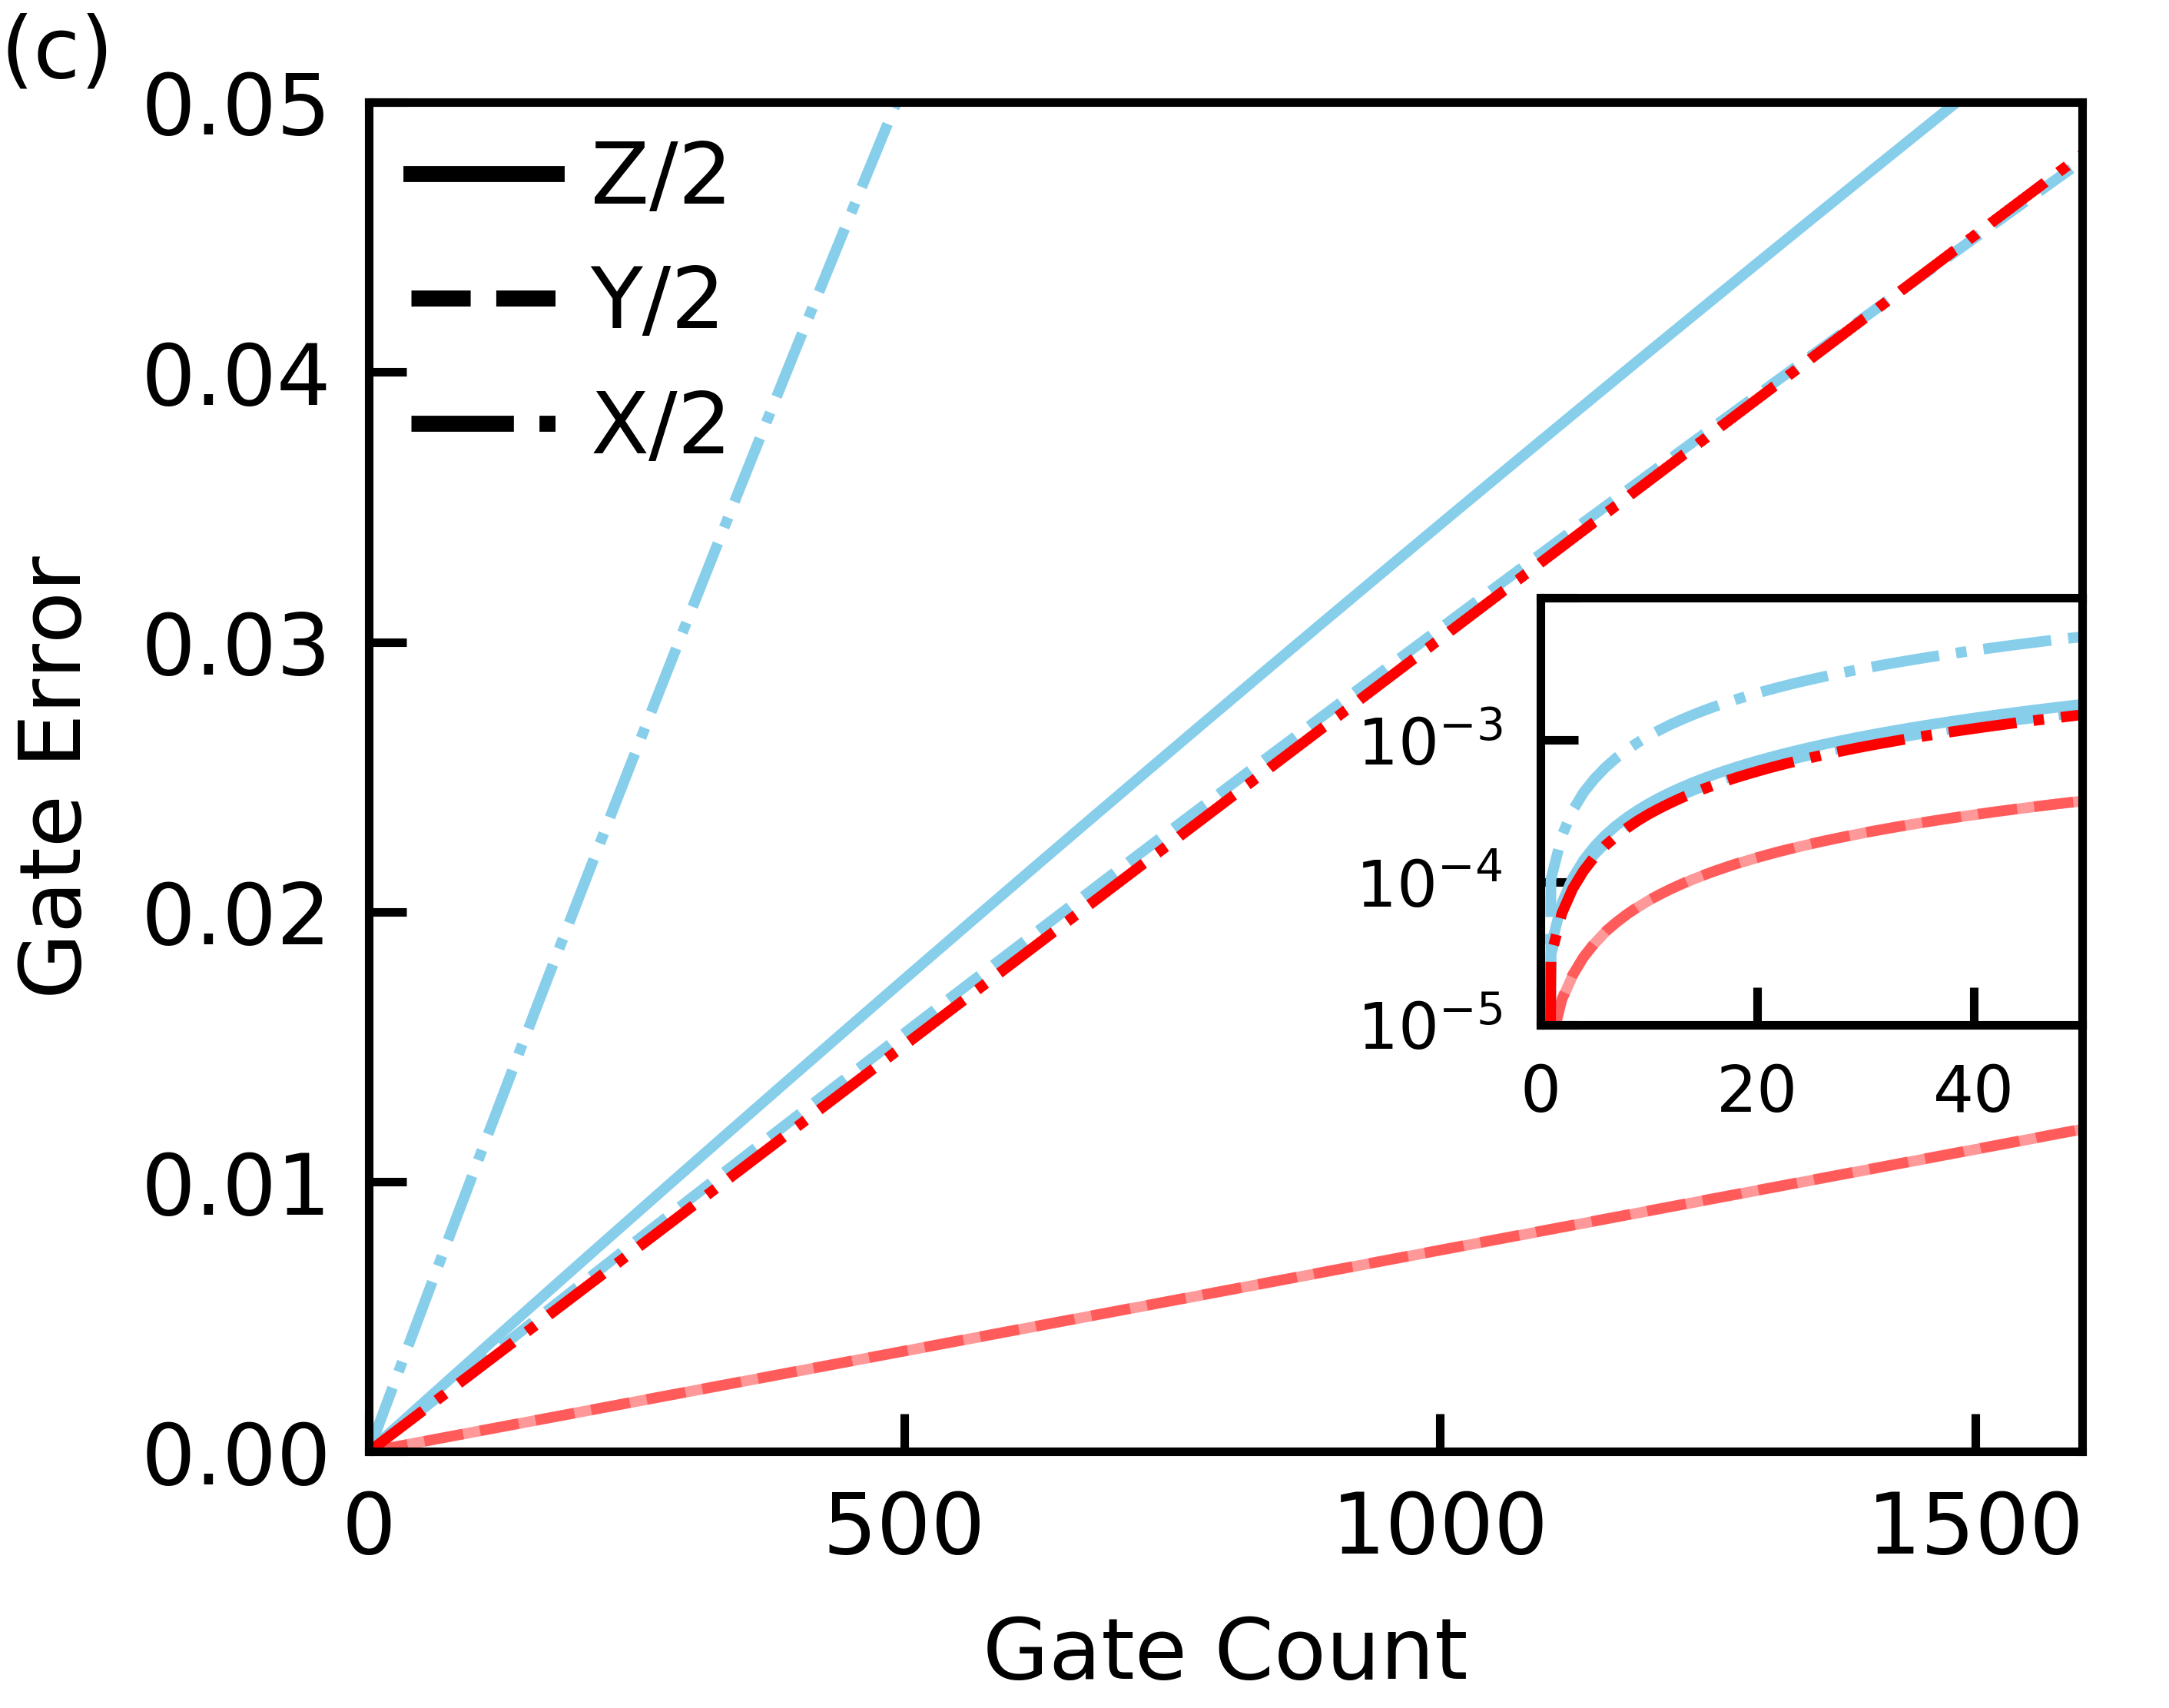
\includegraphics[width=\linewidth]{assets/f1c.png}
  \end{subfigure}
  \caption{
    (a) Numerically optimized gates (red) and analytically optimized gates (blue).
    (b) $T_{1}$ interpolation function used in optimization. Markers
    denote the time-averaged, absolute amplitude of each gate.
    (c) Lindblad master equation simulation with $T_{1}$ dissipation
    for successive gate applications. The reported gate error is the cumulative
    gate error after each gate application.
    The numerically optimized $Z/2$ and $Y/2$ gate errors are indistinguishable
    in the figure.
  }
  \label{fig:longitude}
\end{figure*}

\section{Longitudinal Relaxation Awareness}
The longitudinal relaxation time $T_{1}$ varies with
control parameters in a range of superconducting circuit platforms.
It is advantageous to tune the controls to extend the longitudinal
relaxation time.
Computing the gate error due to longitudinal relaxation
requires propagating density matrices of size $n \times n$ under master equation
dynamics, rather than state vectors of size $n$ under the TDSE dynamics.
We avoid this increase in computational complexity by
penalizing the integrated rate of longitudinal relaxation,
i.e. the probability of longitudinal relaxation.
Using this probability as proxy for the gate error incurred
is reasonable because losses due to longitudinal relaxation
increase monotonically in time.
This technique can be extended to
error channels which share the monotonically increasing property.
Additionally, for a constant $T_{1}$ time, a shorter gate duration
would favor a lower longitudinal relaxation probability. We allow
the optimizer to tune the gate duration in order to minimize the
longitudinal relaxation probability. Our scheme for time-optimal
control is applicable to any time-optimal problem, not only
the one we study here.

The longitudinal relaxation probability is given by
\begin{equation}
  P_{1}(t) = \int_{0}^{t} T_{1}^{-1}(a(t^{\prime})) dt^{\prime}
\end{equation}
$P_{1}$ is penalized using a quadratic cost at each knot point
${\lvert P_{1}(t_{k}) \rvert}^{2}$.
$T_{1}(a_{k})$ is obtained at each knot point by evaluating
a spline fit to experimental data of the form $\{(a, T_{1})\}$.
It is also possible to use a spline fit to theoretically obtained data.
However, $T_{1}$ values are known to fluctuate greatly
with laboratory temperatures \cite{klimov2018fluctuations}.
Interpolating $T_{1}$ from experimental data
increases the fridge truth of the simulation.

We allow the optimizer to tune the gate duration by
making the time step between each knot point $\Delta t_{k}$
a decision variable. Promoting $\Delta t_{k}$ to a decision variable, rather
than the number of knot points $N$, preserves the
Markovian decision structure of the trajectory
optimization problem. To ensure numerical
integration accuracy is maintained we add a bound
constraint at each knot point
$5\textrm{e-}2 \ \textrm{ns} \le
\Delta t_{k} \le 2\textrm{e-}1 \ \textrm{ns}$.
This bound constraint may be
violated for intermediate iterations of the optimization,
so we add the square root of the time step $\sqrt{\Delta t_{k}}$
to the augmented control vector and use the squared root
of the time step $\lvert \Delta t_{k} \rvert$ in optimization.

%% F2
\begin{figure*}[ht]
  \begin{subfigure}{.315\textwidth}
    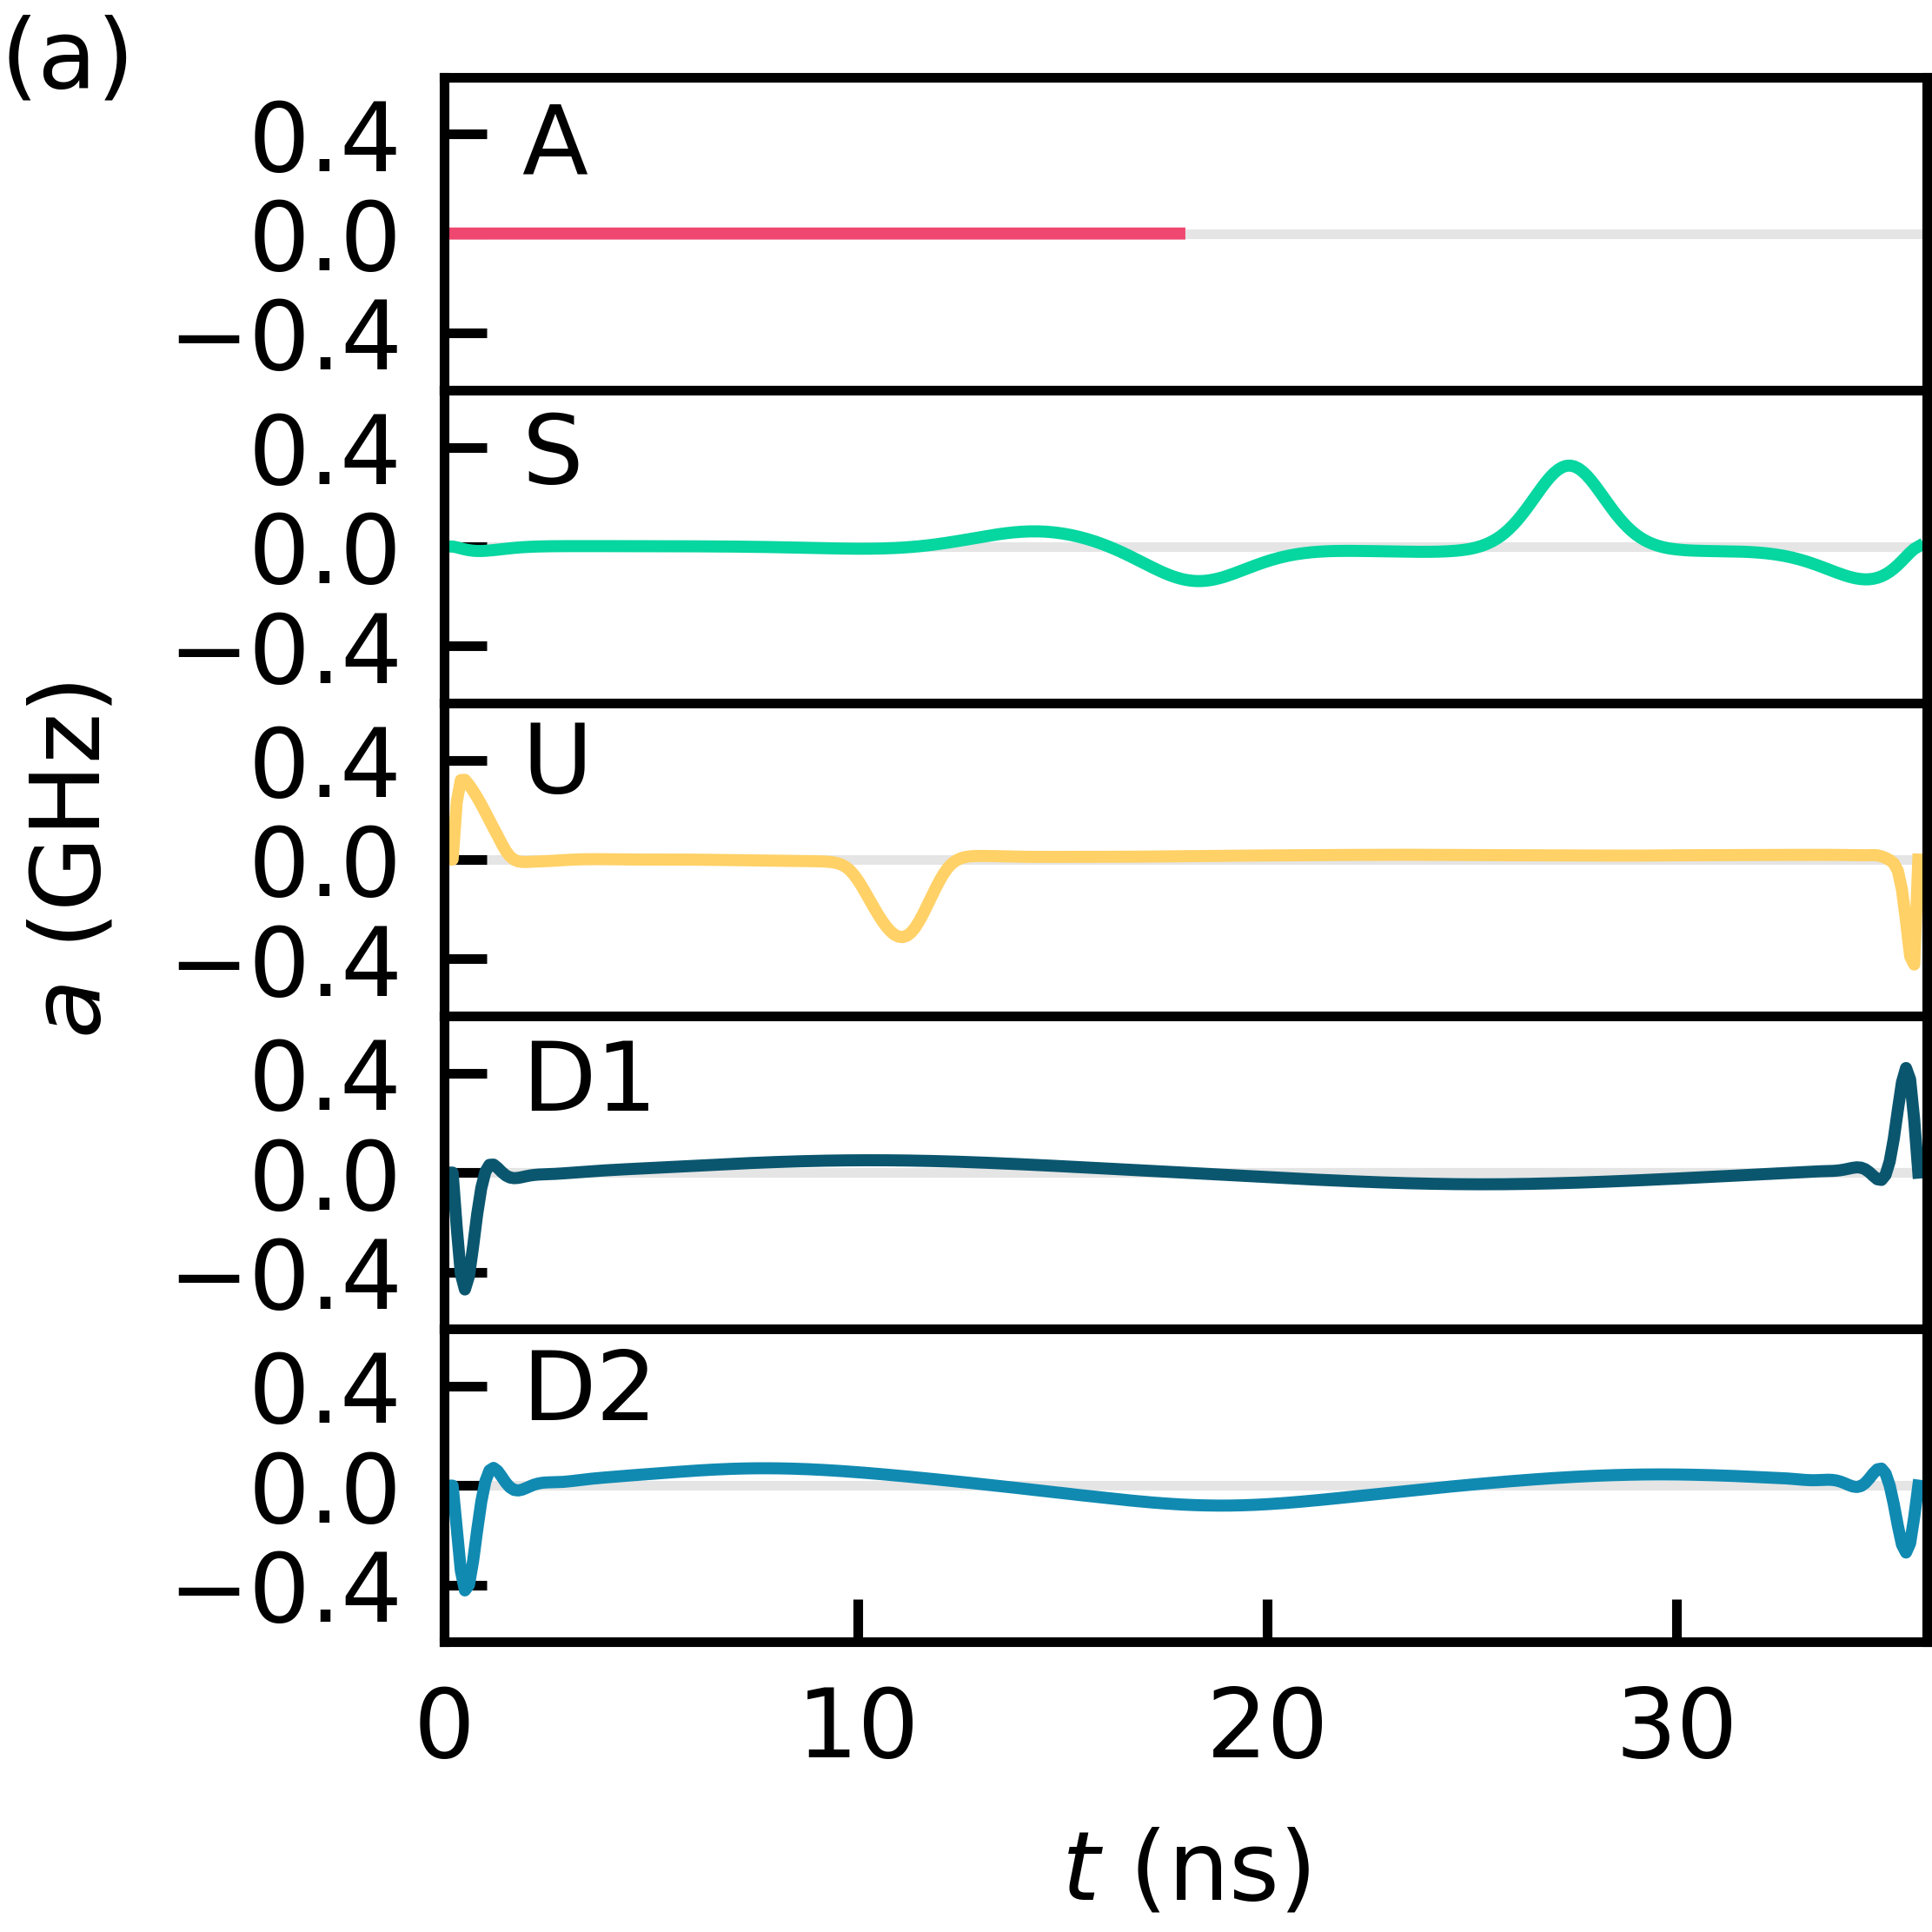
\includegraphics[width=\linewidth]{assets/f2a.png}
  \end{subfigure}\hfill
  \begin{subfigure}{.4\textwidth}
    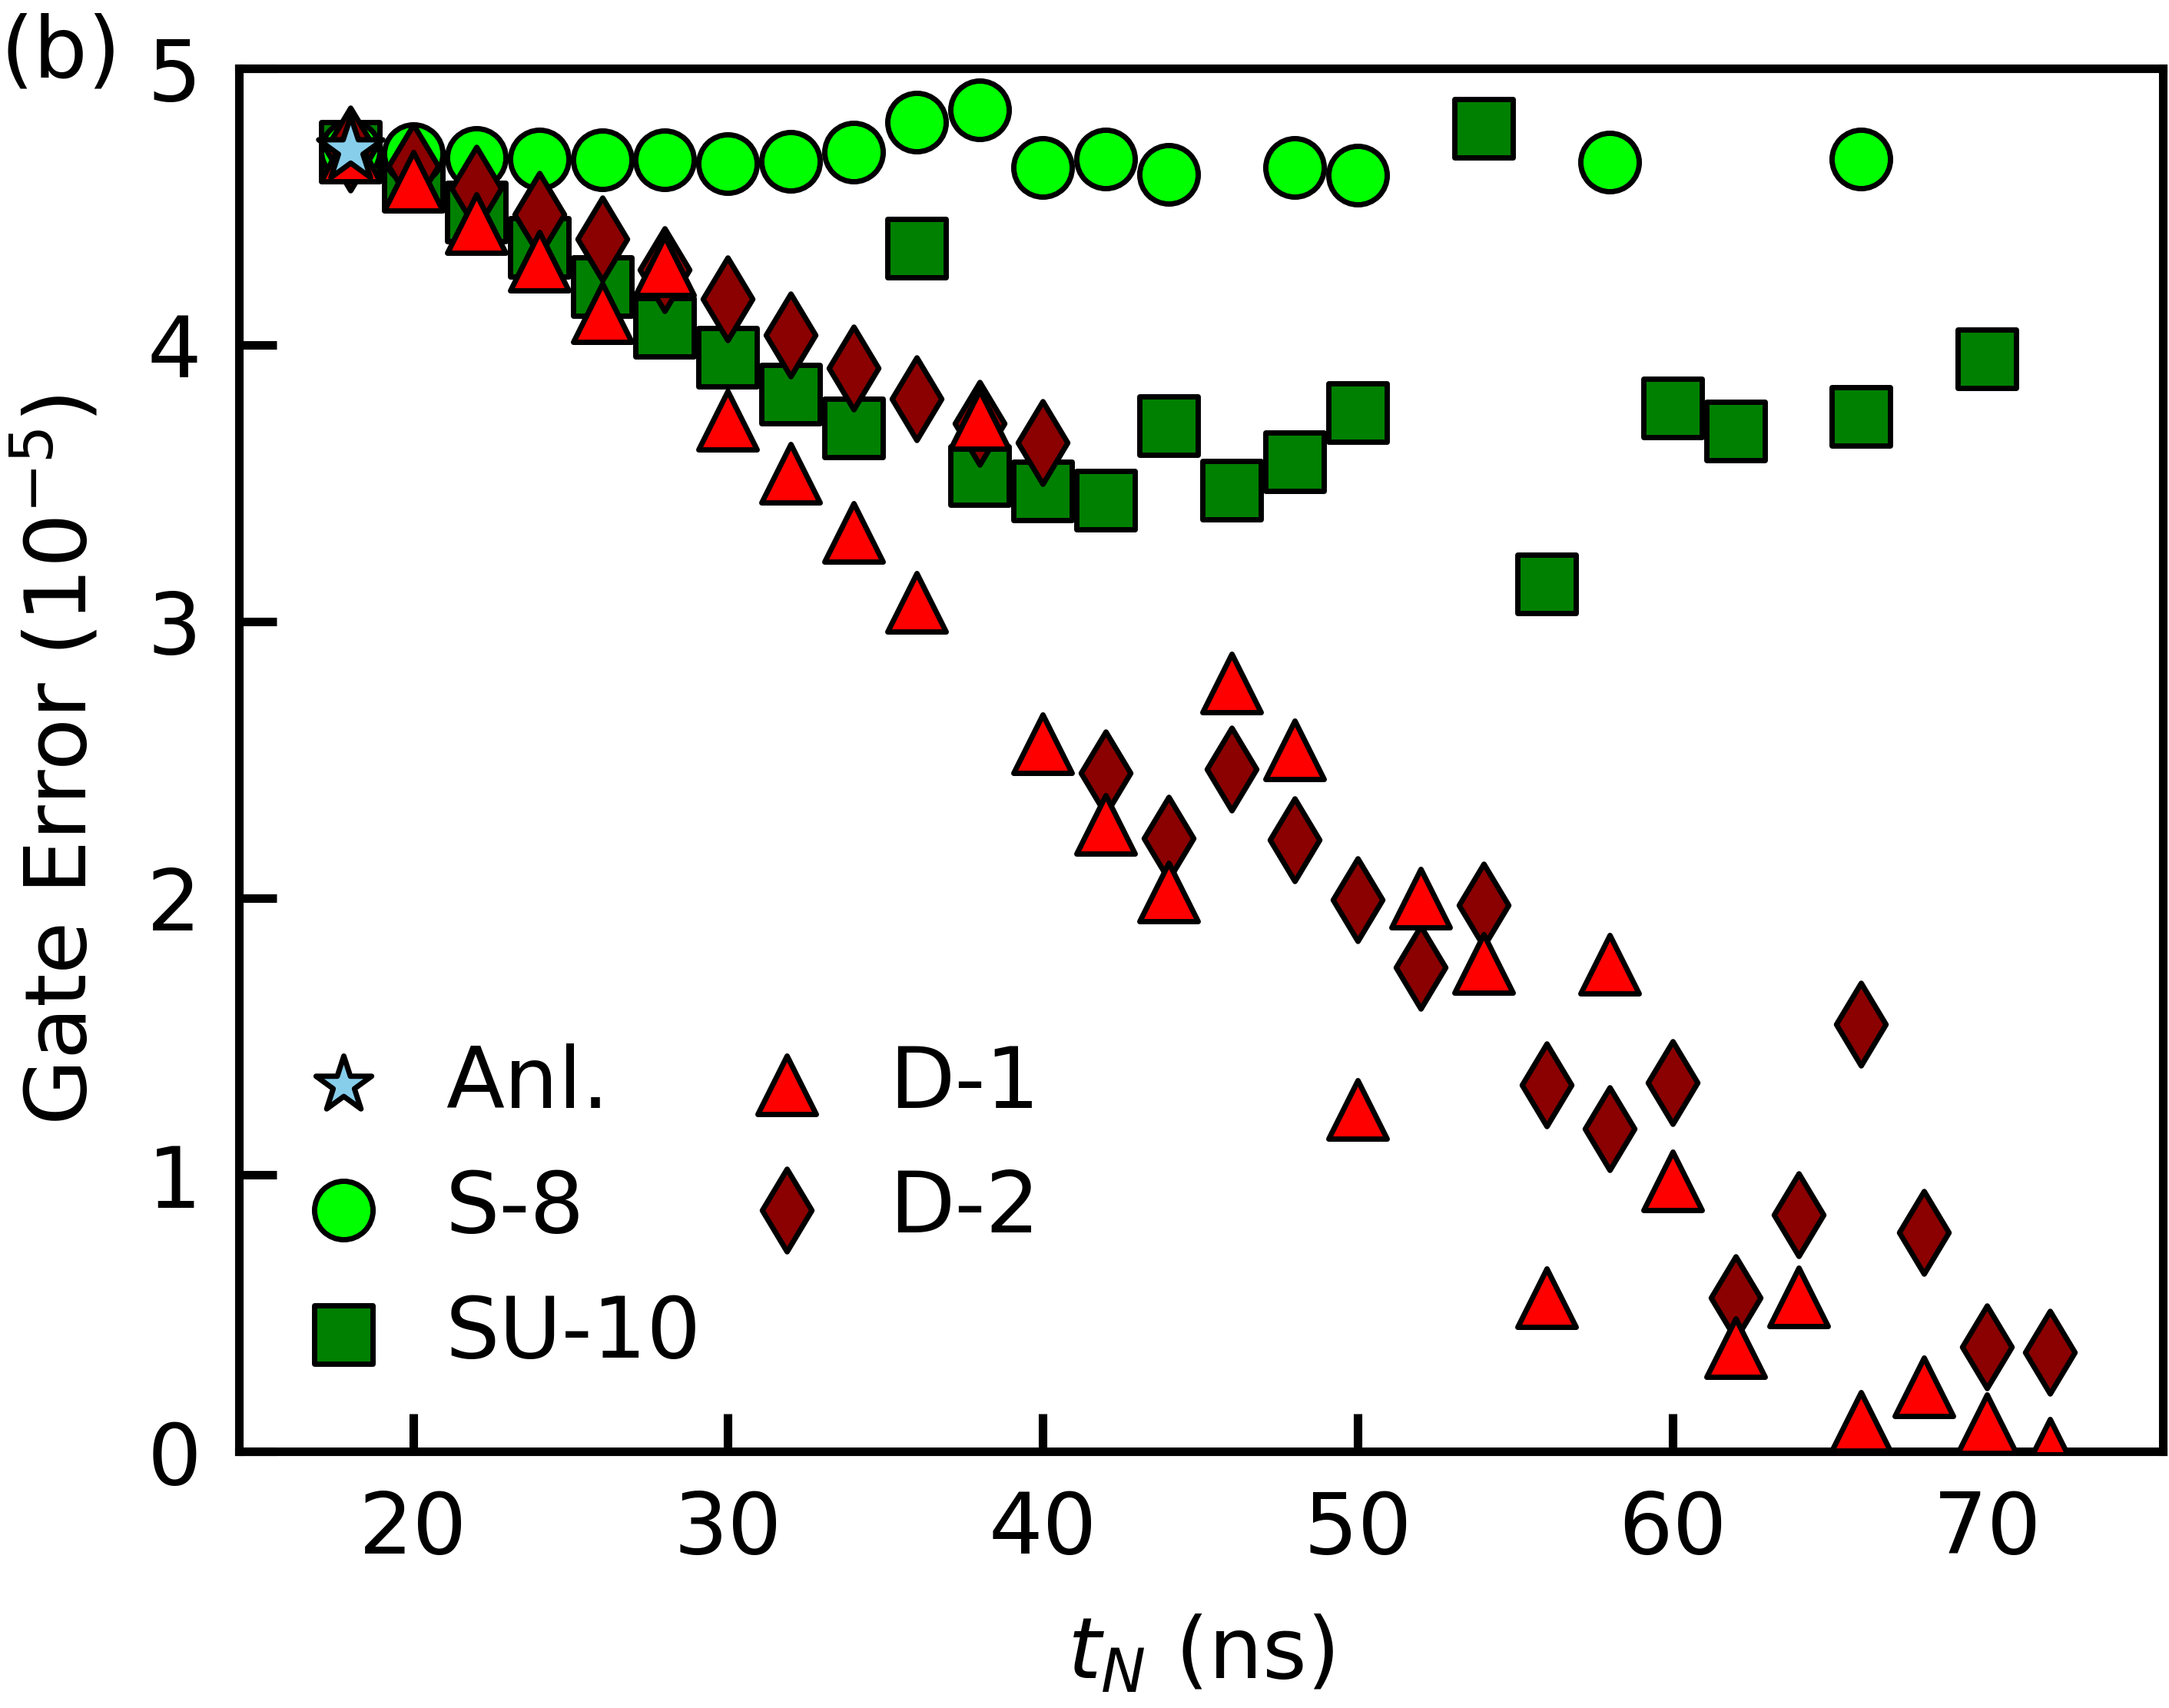
\includegraphics[width=\linewidth]{assets/f2c.png}
  \end{subfigure}\hfill
  \begin{subfigure}{.23\textwidth}
    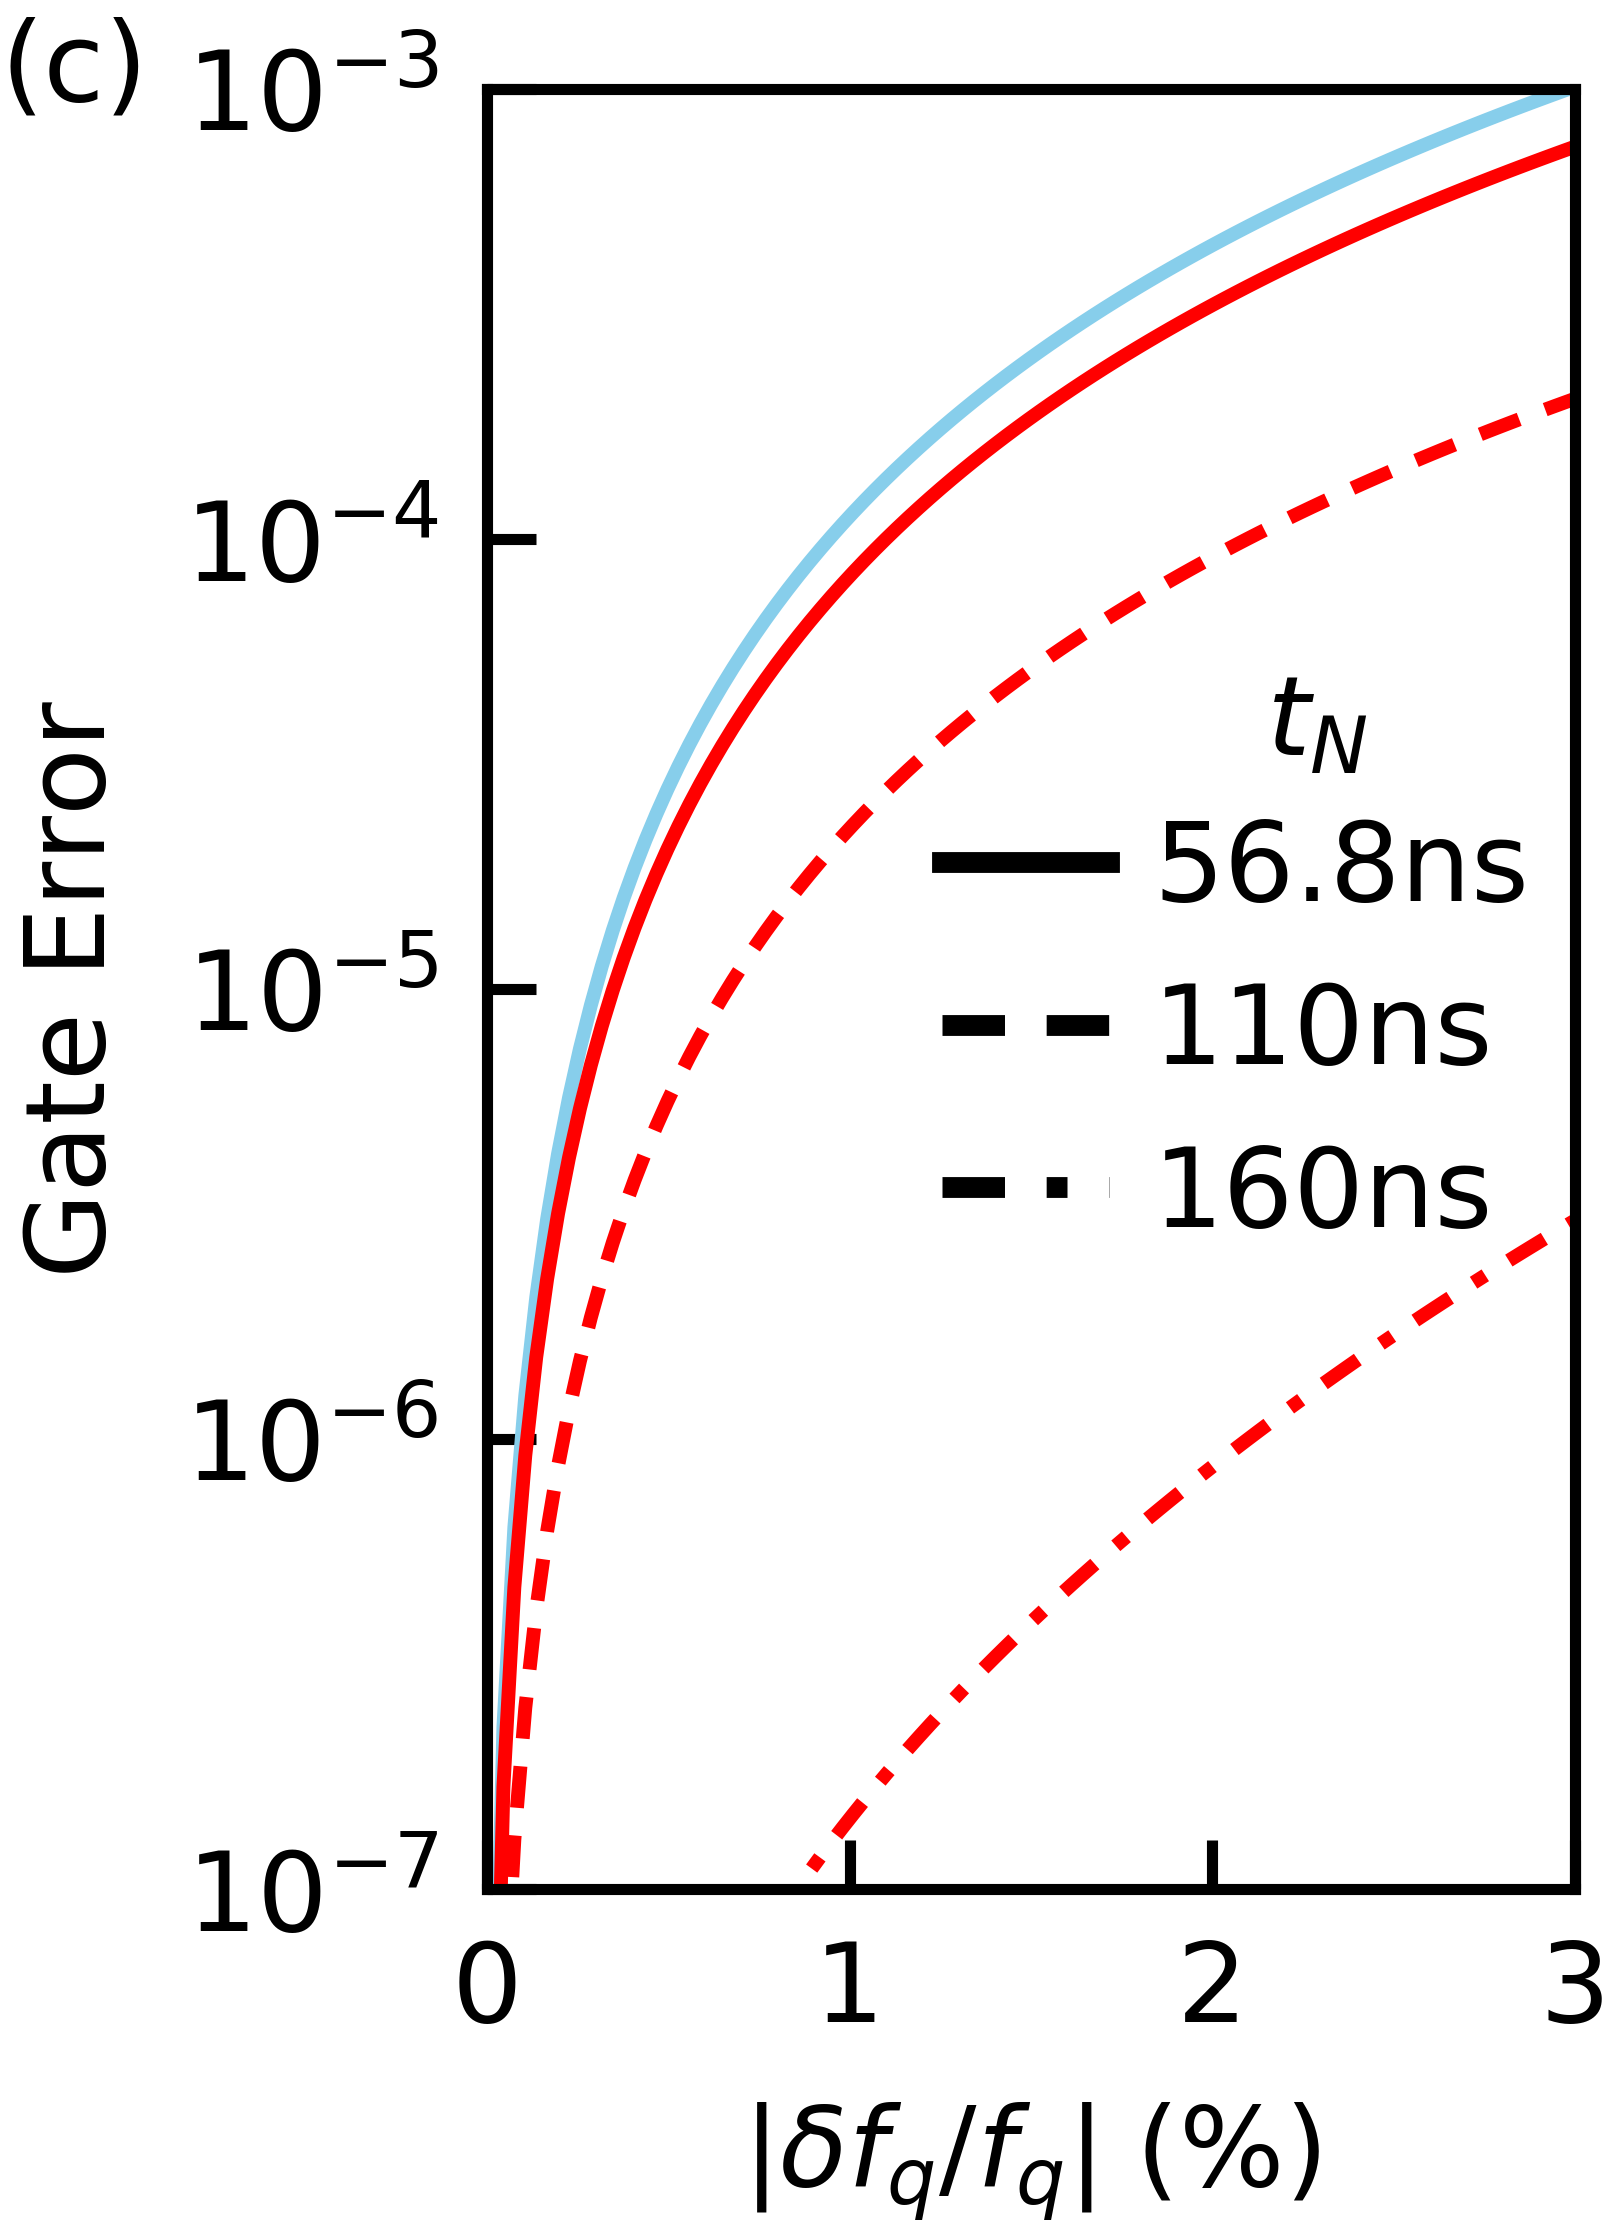
\includegraphics[width=\linewidth]{assets/f2b.png}
  \end{subfigure}
  \caption{
    (a) $Z/2$ gates robust to qubit frequency detunings constructed with the
    analytic, sampling, unscented sampling, and the 1\textsuperscript{st}-
    and 2\textsuperscript{nd}-order derivative methods. The gates
    shown for the numerical methods are the solutions at twice the analytic
    gate time.
    (b) Single gate error as
    a function of the gate duration at a one-percent
    detuning from the nominal qubit frequency for all methods. Missing
    data points represent solutions with a gate error above $5 \cdot 10^{-5}$.
    (c) Single gate error as a function of the detuning from the nominal
    qubit frequency. The solutions for the analytic and
    1\textsuperscript{st}-order derivative methods are shown at multiples
    of the analytic gate time. The performance of the two methods is
    indistinguishable at the analytic gate time $18$ns.
  }
  \label{fig:static}
\end{figure*}

We compare the numerical method we have developed to the analytic gates
on the task of achieving low gate errors in the presence of longitudinal relaxation
for the $Z/2$, $Y/2$, and $X/2$ gates.
The numerically optimized gates converge on similar solutions, a periodic
waveform with amplitude $\sim 0.2 \textrm{GHz}$, see Figure \ref{fig:longitude}.
They extend their gate times
beyond their analytic counterparts, trading longer gate times for access
to higher amplitudes and therefore higher $T_{1}$ times. All numerical gates reduce
their single gate errors by a factor of $5$ over
their analytic counterparts which is commensurate to their
probability of longitudinal relaxation reductions, see Appendix \ref{appendix:longitude}.
The gate error reported in this text is the infidelity
of the evolved state and the target state averaged over 1000 pseudo-randomly
generated initial states. The numerical $Z/2$ and $Y/2$ gates perform simlarly in
the concatenated gate application comparision, suppressing accumulated gate errors to $8 \cdot 10^{-3}$
over $2000$ gate applications $\sim 40 \mu\textrm{s}$. The numerical $X/2$ gate
achieves an accumulated gate error of $1.7 \cdot 10^{-2}$ over $2000$ gate applications $\sim 124 \mu\textrm{s}$.
Both the analytic and numerical gates attain single gate errors sufficient for
quantum error correction $< 10^{-4}$, requisite for fault-tolerant quantum computing.
The low gate errors achieved by the numerical gates for extend computations
are critical for noisy, intermediate-scale quantum (NISQ) applications.
These improvements are significant for the realistic constraints we have imposed
on the gates, and do not represent a fundamental limit to the optimization methods we have
employed.

